% =====================================================================
% IBFE Tutorials: using Planktos
% API audited against Planktos v1.0.3, commit a1c2128 (2026-08-19)
% =====================================================================
\documentclass[aspectratio=169,11pt]{beamer}

% Match the visual language of the SIAM Waves talk.
\usetheme{Boadilla}
\usecolortheme{seahorse}
\useinnertheme{rectangles}
\useoutertheme{infolines}

\setbeamercolor{structure}{fg=blue!55!black}
\setbeamercolor{title}{fg=white,bg=blue!55!black}
\setbeamercolor{frametitle}{fg=blue!55!black}
\setbeamercolor{block title}{bg=blue!12,fg=blue!55!black}
\setbeamercolor{block body}{bg=blue!4}
\setbeamercolor{alertblock title}{bg=orange!22,fg=orange!55!black}
\setbeamercolor{alertblock body}{bg=orange!5}
\setbeamertemplate{navigation symbols}{}
\setbeamerfont{frametitle}{series=\bfseries,size=\large}
\setbeamerfont{title}{series=\bfseries,size=\Large}

\usepackage[T1]{fontenc}
\usepackage[utf8]{inputenc}
\DeclareFontShape{T1}{cmss}{b}{n}{<->ssub*cmss/bx/n}{}
\usepackage{amsmath,amssymb,bm,mathtools}
\usepackage{booktabs,array}
\usepackage{graphicx}
\usepackage{xcolor}
\usepackage{tikz}
\usetikzlibrary{arrows.meta,calc,positioning,fit}
\usepackage{listings}
\usepackage{tcolorbox}
\tcbuselibrary{skins}
\usepackage{hyperref}

\hypersetup{colorlinks=true,urlcolor=blue!55!black}
\graphicspath{{pictures/6-planktos/}{../pictures/6-planktos/}}

\definecolor{plankblue}{RGB}{38,86,145}
\definecolor{plankteal}{RGB}{28,132,132}
\definecolor{plankgreen}{RGB}{53,128,95}
\definecolor{plankorange}{RGB}{208,112,44}
\definecolor{plankgray}{RGB}{92,101,112}
\definecolor{codebg}{RGB}{247,249,252}

\newcommand{\hi}[1]{\textcolor{blue!55!black}{\textbf{#1}}}
\newcommand{\soft}[1]{\textcolor{gray!55!black}{#1}}
\newcommand{\vect}[1]{\bm{#1}}
\newcommand{\source}[1]{\par\vspace{1pt}{\tiny\color{gray!65!black}#1}}

\newtcolorbox{punchbox}{
  enhanced,
  colback=blue!4,
  colframe=blue!55!black,
  boxrule=0.6pt,
  arc=2pt,
  left=4pt,right=4pt,top=3pt,bottom=3pt
}

\lstdefinestyle{plankpy}{
  language=Python,
  basicstyle=\ttfamily\fontsize{7.2}{8.0}\selectfont,
  keywordstyle=\color{plankblue}\bfseries,
  commentstyle=\color{plankgreen!80!black},
  stringstyle=\color{plankorange!85!black},
  showstringspaces=false,
  columns=fullflexible,
  keepspaces=true,
  breaklines=true,
  breakatwhitespace=true,
  frame=single,
  rulecolor=\color{blue!18},
  backgroundcolor=\color{codebg},
  xleftmargin=3pt,
  xrightmargin=3pt,
  aboveskip=3pt,
  belowskip=3pt
}
\lstset{style=plankpy}

\title[Using Planktos]{Using Planktos}
\subtitle{Agent-based transport and behavior in fluid environments}
\author[Miller]{Laura A. Miller}
\institute[UArizona]{Department of Mathematics, University of Arizona}
\date{}

\begin{document}

% ----- 1. Title -----
\begin{frame}[plain]
  \begin{beamercolorbox}[sep=10pt,center]{title}
    {\bfseries\Large Using Planktos}\\[3pt]
    {\normalsize Agent-based transport and behavior in fluid environments}
  \end{beamercolorbox}
  \vspace{0.7em}
  \begin{columns}[T,onlytextwidth]
  \begin{column}{0.47\textwidth}
    \textbf{\large Laura A. Miller}\\[4pt]
    Department of Mathematics\\
    University of Arizona\\[8pt]
    {\small IBFE Tutorials}\\[8pt]
    \parbox{0.98\linewidth}{\tiny AI tools were used to assist with formatting, organization, and clarification of the instructor's original notes.}
  \end{column}
  \begin{column}{0.50\textwidth}
    \centering
    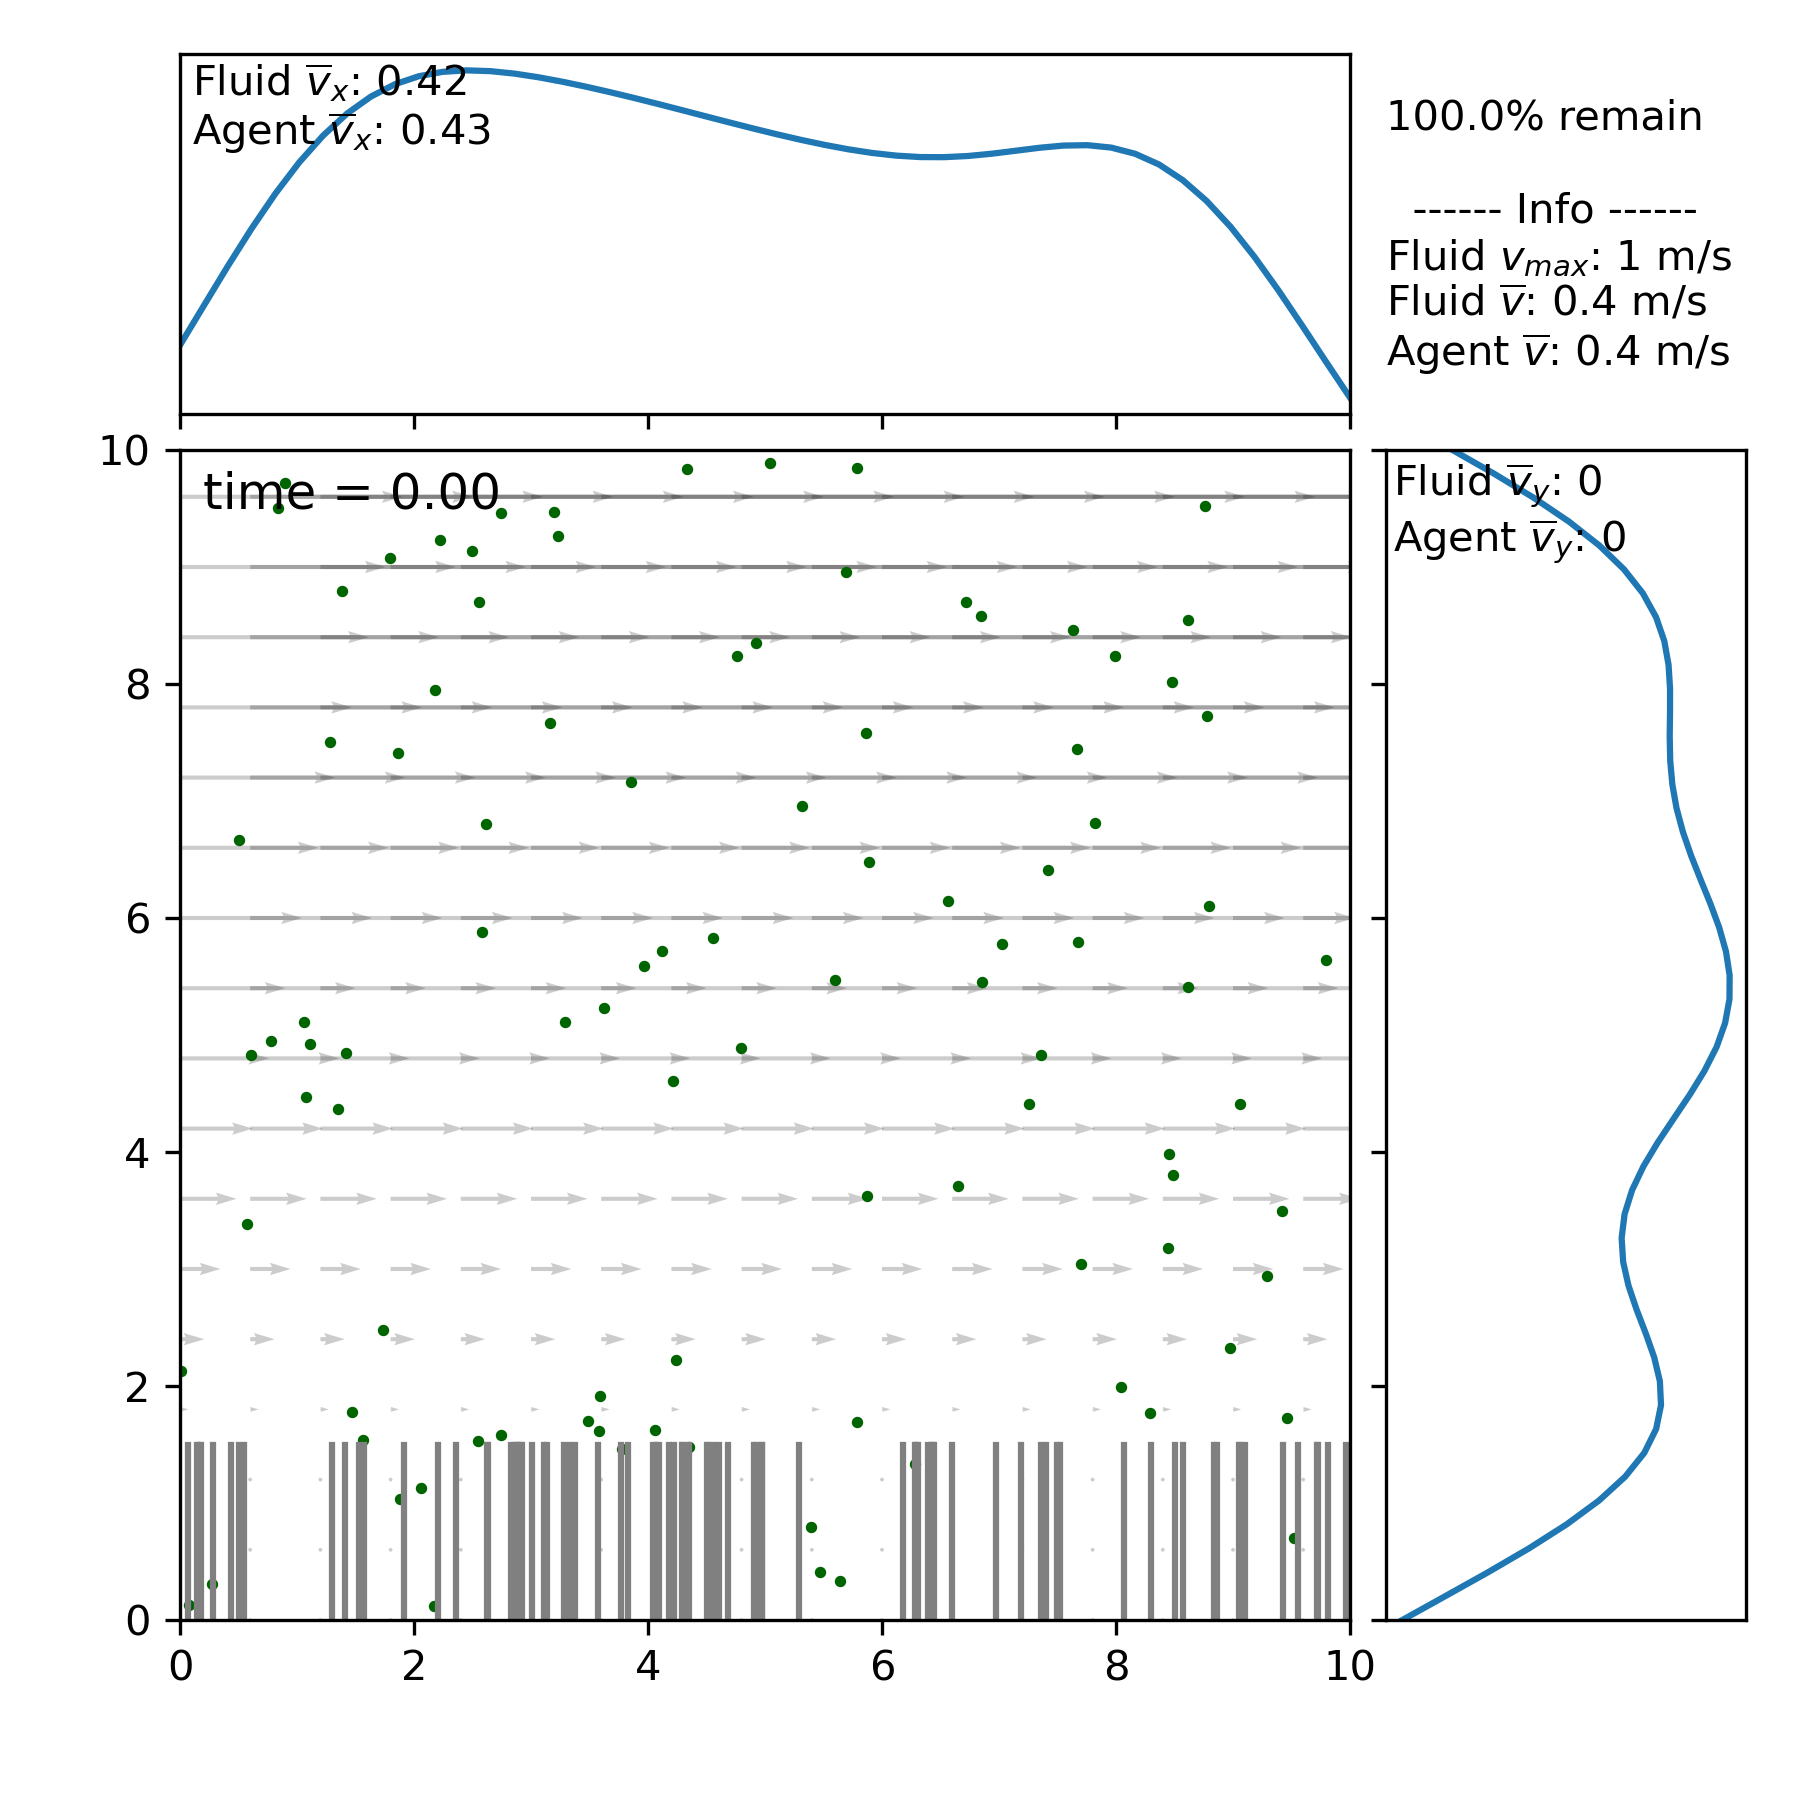
\includegraphics[width=\linewidth,height=0.50\textheight,keepaspectratio]{repo-basic-2d-agents.png}
    \source{Planktos documentation image \texttt{docs/\_static/basic\_ex\_2d\_agents.png} (commit \texttt{a1c2128}, GPLv3).}
  \end{column}
  \end{columns}
\end{frame}

% ----- 2. Goals -----
\begin{frame}{What you will be able to build}
\begin{columns}[T,onlytextwidth]
\begin{column}{0.48\textwidth}
\begin{block}{Core workflow}
\begin{itemize}\itemsep2pt
  \item create a 2D or 3D \texttt{Environment};
  \item specify outer-domain boundary conditions;
  \item generate or import a velocity field and mesh;
  \item initialize one or more vectorized \texttt{Swarm}s;
  \item advance, inspect, plot, animate, and export.
\end{itemize}
\end{block}
\end{column}
\begin{column}{0.48\textwidth}
\begin{block}{Research extensions}
\begin{itemize}\itemsep4pt
  \item encode deterministic, stochastic, or social behavior;
  \item choose sliding, sticky, or disabled mesh collisions;
  \item compute KDE and finite-time Lyapunov exponent fields;
  \item reproduce a current Vicsek-model example.
\end{itemize}
\end{block}
\end{column}
\end{columns}
\begin{punchbox}
\footnotesize
\centering
Every code fragment targets \textbf{Planktos v1.0.3}, repository commit \texttt{a1c2128} (2026-08-19). Unless a slide explicitly continues prior state, treat each fragment as a separate pattern in a fresh environment.
\end{punchbox}
\end{frame}

% ----- 3. Scope -----
\begin{frame}{Modeling scope: agents respond to a prescribed flow}
\small
\begin{columns}[T,onlytextwidth]
\begin{column}{0.52\textwidth}
Planktos is designed for point-particle organisms or particles whose feedback on the surrounding flow is negligible. A useful template is
\[
  d\vect X
  = \big[\vect u(\vect X,t)+\vect b(\vect X,t;\theta)\big]dt
    + \boldsymbol{\sigma}\,d\vect W_t ,
\]
\begin{itemize}\itemsep2pt
  \item \(\vect u\): prescribed CFD or analytical velocity field;
  \item \(\vect b\): swimming, settling, taxis, or social drift;
  \item \(\boldsymbol{\sigma}\): stochastic variability, constant in space (it may still differ per agent);
  \item boundaries and immersed meshes constrain the proposed step.
\end{itemize}
{\scriptsize A spatially varying \(\boldsymbol\sigma(\vect X)\) needs a Milstein-type scheme; the built-in Euler--Maruyama step is only order 0.5 in that case and does not support it directly.}
{\footnotesize\textcolor{red!75!black}{\textbf{One-way coupling.}}
Agent motion does \emph{not} alter \(\vect u\); use a coupled solver when feedback matters.}
\end{column}
\begin{column}{0.45\textwidth}
\centering
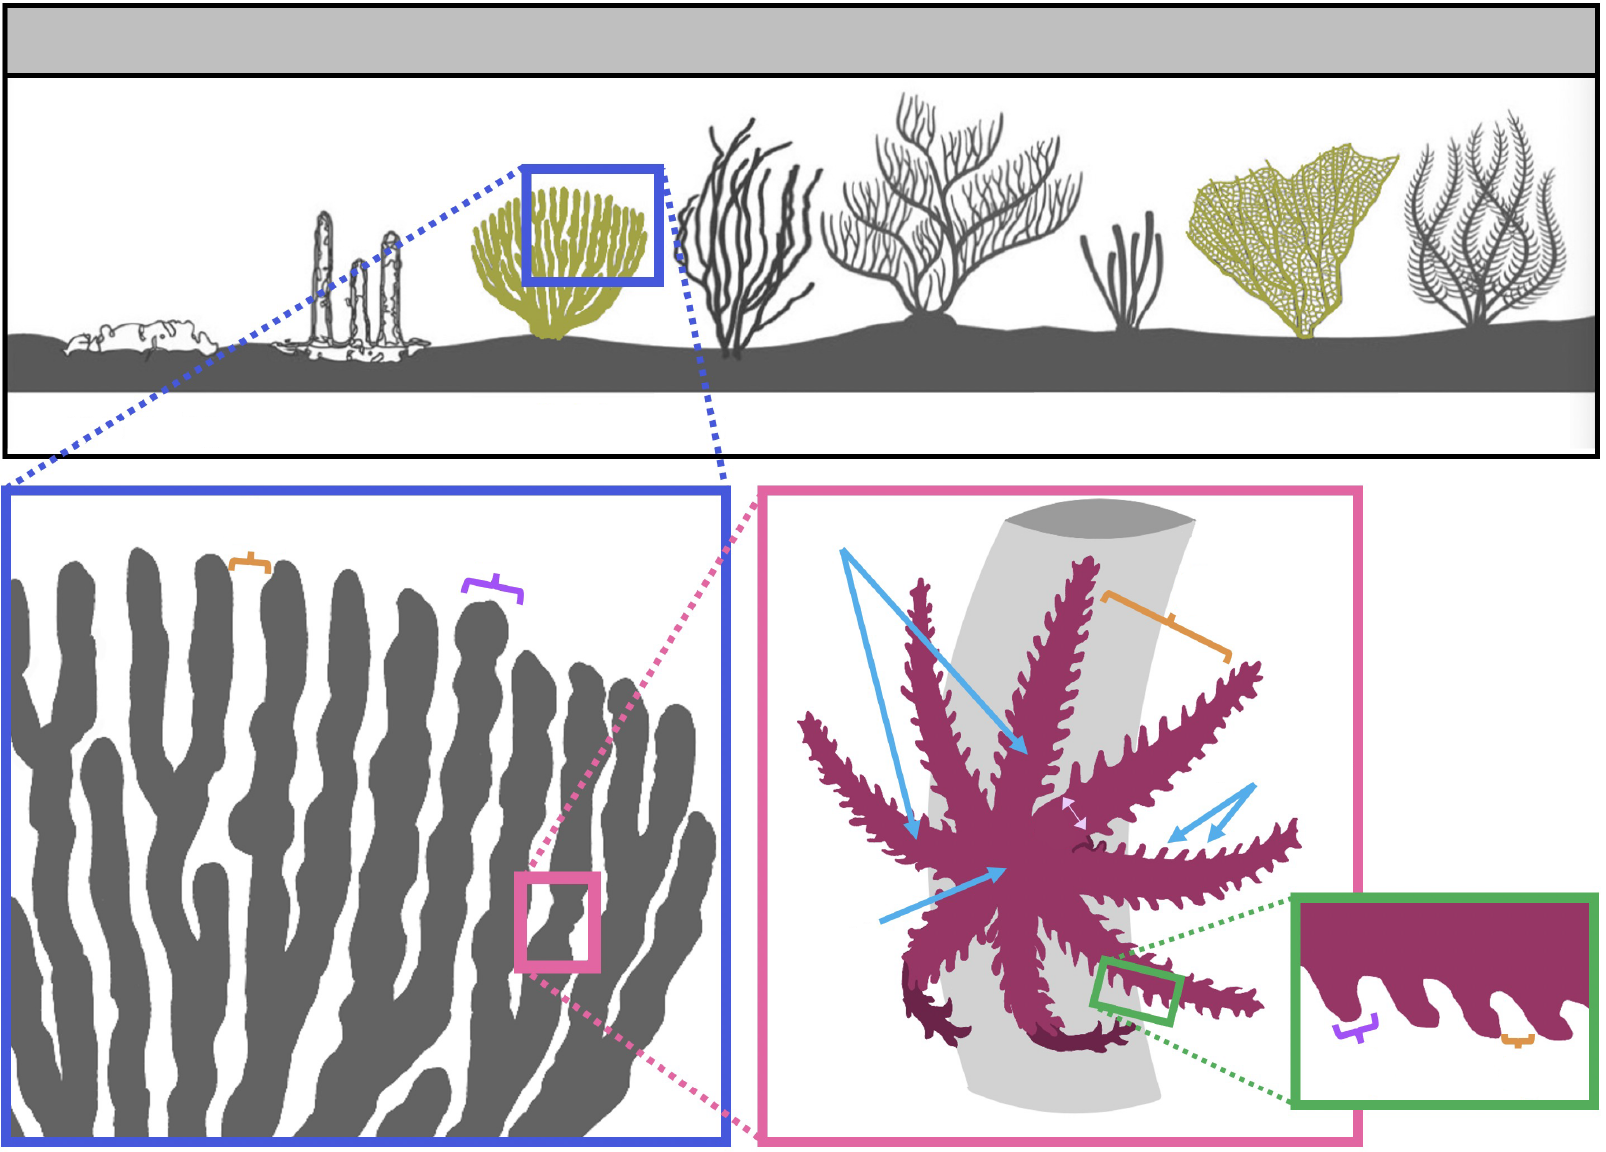
\includegraphics[width=\linewidth,height=0.48\textheight,keepaspectratio]{jeb2023-fig1-gorgonian-scales.png}
\source{Biological scales and gorgonian morphology: Hamlet et al. (2023), Fig.~1 (adapted from Kupfner Johnson \& Hallock, 2020), CC BY 4.0.}
\end{column}
\end{columns}
\end{frame}

% ----- 4. Workflow -----
\begin{frame}{The end-to-end workflow}
\centering
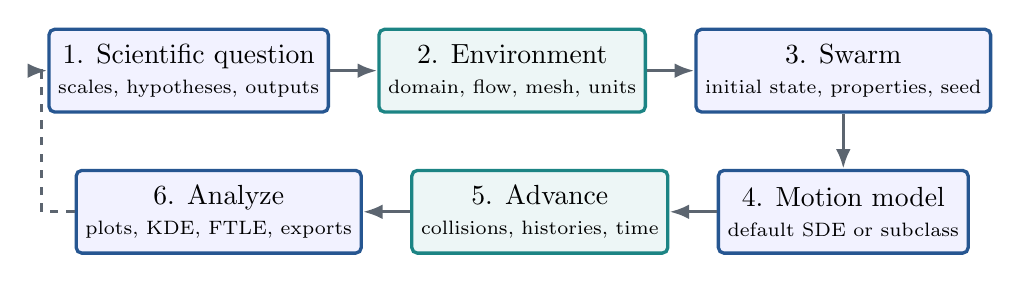
\begin{tikzpicture}[
  node distance=7mm and 6mm,
  box/.style={draw=plankblue,very thick,rounded corners=2pt,fill=blue!5,
              minimum width=3.0cm,minimum height=1.05cm,align=center},
  data/.style={draw=plankteal,very thick,rounded corners=2pt,fill=teal!7,
               minimum width=3.0cm,minimum height=1.05cm,align=center},
  arr/.style={-{Latex[length=2.5mm]},very thick,plankgray}
]
\node[box] (question) {1. Scientific question\\[-1pt]\scriptsize scales, hypotheses, outputs};
\node[data,right=of question] (flow) {2. Environment\\[-1pt]\scriptsize domain, flow, mesh, units};
\node[box,right=of flow] (agents) {3. Swarm\\[-1pt]\scriptsize initial state, properties, seed};
\node[box,below=of agents] (behavior) {4. Motion model\\[-1pt]\scriptsize default SDE or subclass};
\node[data,left=of behavior] (advance) {5. Advance\\[-1pt]\scriptsize collisions, histories, time};
\node[box,left=of advance] (analyse) {6. Analyze\\[-1pt]\scriptsize plots, KDE, FTLE, exports};
\draw[arr] (question)--(flow);
\draw[arr] (flow)--(agents);
\draw[arr] (agents)--(behavior);
\draw[arr] (behavior)--(advance);
\draw[arr] (advance)--(analyse);
\draw[arr,dashed] (analyse.west) -- ++(-0.42,0) |- (question.west);
\end{tikzpicture}
\vspace{0.8em}
\begin{punchbox}
\centering
Treat plotting and diagnostics as part of the simulation loop: inspect early, then scale up.
\end{punchbox}
\end{frame}

% ----- 5. Install -----
\begin{frame}[fragile]{Install from the cloned repository}
Clone the official repository, then make an isolated environment inside it.
\begin{lstlisting}
git clone https://github.com/mountaindust/Planktos.git
cd Planktos
python -m venv .venv

# PowerShell
.\.venv\Scripts\Activate.ps1
# macOS/Linux: source .venv/bin/activate

python -m pip install --upgrade pip
python -m pip install -e .
python -c "import planktos; print(planktos.__version__)"
\end{lstlisting}
Expected version for this deck: \texttt{1.0.3}.

\begin{columns}[T,onlytextwidth]
\begin{column}{0.48\textwidth}
\begin{block}{Editable install}
\texttt{-e} points the environment at the clone, so a later \texttt{git pull} updates the import without reinstalling.
\end{block}
\end{column}
\begin{column}{0.48\textwidth}
\begin{block}{Smoke test}
Run \texttt{python examples/basic\_ex\_2d.py}; close each interactive plot to continue.
\end{block}
\end{column}
\end{columns}
\source{Adapted from the repository \texttt{README.md} Quickstart.}
\end{frame}

% ----- 6. Dependencies -----
\begin{frame}[fragile]{Dependencies: what is installed, and what is optional}
\small
\begin{columns}[T,onlytextwidth]
\begin{column}{0.57\textwidth}
\begin{tabular}{@{}p{0.30\linewidth}p{0.62\linewidth}@{}}
\toprule
\textbf{Declared core} & \textbf{Role} \\
\midrule
Python \(\ge 3.8\) & runtime (development currently uses newer Python) \\
NumPy \(\ge 1.19\) & vectorized agent and field arrays \\
SciPy \(\ge 1.10.1\) & interpolation, KDE, ODE integration \\
Matplotlib \(\ge 3.0\) & plots and animations \\
pandas & per-agent properties \\
VTK/PyVista & \(\ge 9.2/\ge 0.44\); CFD/mesh I/O and VTK output \\
\bottomrule
\end{tabular}
\end{column}
\begin{column}{0.39\textwidth}
\begin{block}{Optional extras}
\begin{lstlisting}
python -m pip install -e ".[STL,netCDF,test]"
\end{lstlisting}
\begin{itemize}\itemsep2pt
  \item \texttt{numpy-stl}: STL input;
  \item \texttt{netCDF4}: NetCDF input;
  \item \texttt{pytest}: test suite.
\end{itemize}
\end{block}
\begin{alertblock}{VTK installation}
If binary resolution becomes difficult, the project documentation recommends a clean conda-forge/Miniforge environment.
\end{alertblock}
\end{column}
\end{columns}
\source{Versions and extras are from \texttt{setup.cfg} at commit \texttt{a1c2128}.}
\end{frame}

% ----- 7. FFmpeg -----
\begin{frame}[fragile]{FFmpeg is needed only when saving animations}
\begin{columns}[T,onlytextwidth]
\begin{column}{0.52\textwidth}
\begin{lstlisting}
# Verify that the executable is on PATH
ffmpeg -version

# PowerShell can also locate it explicitly
Get-Command ffmpeg
\end{lstlisting}
\begin{block}{Without FFmpeg}
Simulations, static plots, and interactive animations still work. A filename passed to \texttt{plot\_all} triggers the external movie writer.
\end{block}
\end{column}
\begin{column}{0.44\textwidth}
\begin{alertblock}{If it is not found}
\begin{enumerate}\itemsep4pt
  \item install FFmpeg with the platform's package manager or official installer;
  \item add its executable directory to \texttt{PATH};
  \item restart the terminal or IDE;
  \item rerun \texttt{ffmpeg -version} in the same environment that runs Python.
\end{enumerate}
\end{alertblock}
\end{column}
\end{columns}
\begin{punchbox}
\centering
For long simulations, save every \(k\)-th state as a frame; rendering every time step is rarely useful.
\end{punchbox}
\end{frame}

% ----- 8. Object model -----
\begin{frame}{Two objects organize almost everything}
\centering
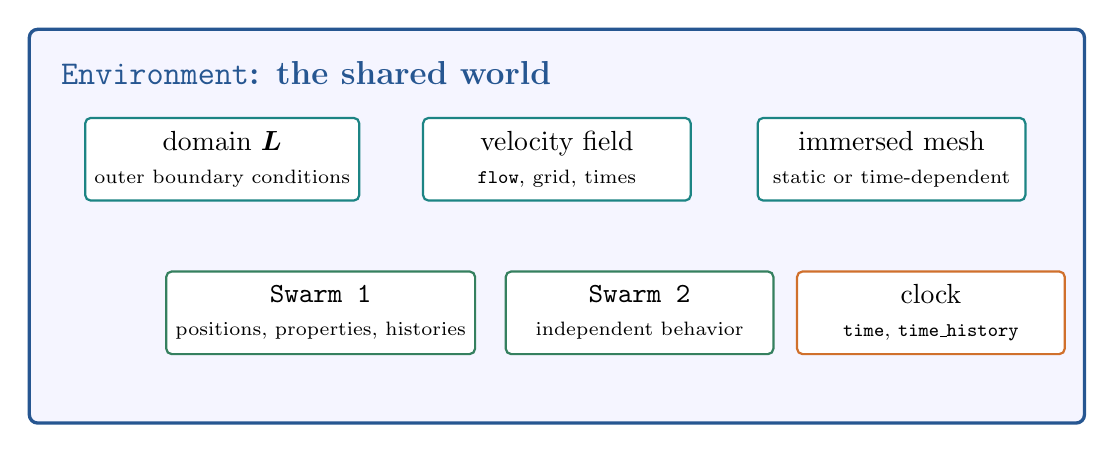
\begin{tikzpicture}[
  outer/.style={draw=plankblue,very thick,rounded corners=3pt,fill=blue!4,
                minimum width=13.4cm,minimum height=5.0cm},
  inner/.style={draw=plankteal,thick,rounded corners=2pt,fill=white,
                minimum width=3.4cm,minimum height=1.05cm,align=center}
]
\node[outer] (env) {};
\node[anchor=north west,font=\bfseries\large,text=plankblue] at ([xshift=3mm,yshift=-3mm]env.north west)
  {\texttt{Environment}: the shared world};
\node[inner] at ([xshift=-4.25cm,yshift=0.85cm]env.center) {domain \(\vect L\)\\\scriptsize outer boundary conditions};
\node[inner] at ([xshift=0cm,yshift=0.85cm]env.center) {velocity field\\\scriptsize \texttt{flow}, grid, times};
\node[inner] at ([xshift=4.25cm,yshift=0.85cm]env.center) {immersed mesh\\\scriptsize static or time-dependent};
\node[inner,draw=plankgreen] at ([xshift=-3.0cm,yshift=-1.10cm]env.center) {\texttt{Swarm 1}\\\scriptsize positions, properties, histories};
\node[inner,draw=plankgreen] at ([xshift=1.05cm,yshift=-1.10cm]env.center) {\texttt{Swarm 2}\\\scriptsize independent behavior};
\node[inner,draw=plankorange] at ([xshift=4.75cm,yshift=-1.10cm]env.center) {clock\\\scriptsize \texttt{time}, \texttt{time\_history}};
\end{tikzpicture}
\vspace{0.55em}
\begin{itemize}\itemsep3pt
  \item A swarm is a vectorized group: agents are rows of NumPy arrays, not separate Python objects.
  \item All swarms in one environment sample the same flow and mesh.
\end{itemize}
\end{frame}

% ----- 9. First Environment -----
\begin{frame}[fragile]{Create the first environment}
\begin{columns}[T,onlytextwidth]
\begin{column}{0.56\textwidth}
\begin{lstlisting}
import planktos

env = planktos.Environment(
    Lx=20, Ly=5,
    x_bndry="zero",
    y_bndry=["noflux", "noflux"],
    rho=1000, mu=1.0,
    units="m")

print(env.L)       # [20, 5]
print(env.nu)      # mu/rho = 0.001
print(env.time)    # 0.0
\end{lstlisting}
\end{column}
\begin{column}{0.40\textwidth}
\begin{block}{Defaults worth knowing}
\begin{itemize}\itemsep4pt
  \item \(10\times10\) two-dimensional domain;
  \item zero velocity everywhere;
  \item \texttt{zero} boundaries in \(x,y\);
  \item no swarms or immersed mesh;
  \item \texttt{time = 0.0}.
\end{itemize}
\end{block}
\begin{alertblock}{Units are metadata}
\texttt{units} does not rescale data automatically. Make the flow, mesh, agent parameters, gravity, and time convention consistent yourself.
\end{alertblock}
\end{column}
\end{columns}
\end{frame}

% ----- 10. Outer boundary conditions -----
\begin{frame}{Outer-domain boundary conditions}
\small
\begin{tabular}{@{}p{0.19\linewidth}p{0.48\linewidth}p{0.25\linewidth}@{}}
\toprule
\textbf{Setting} & \textbf{What happens to an agent crossing the box} & \textbf{Typical use} \\
\midrule
\texttt{zero} & The agent is masked and no longer updated or plotted. & open/outflow boundary \\
\texttt{noflux} & The proposed displacement through the wall is projected along it. & solid outer wall \\
\texttt{periodic} & The agent exits one side and re-enters on the opposite side. & repeating domain \\
\bottomrule
\end{tabular}

\vspace{0.6em}
\begin{columns}[T,onlytextwidth]
\begin{column}{0.53\textwidth}
Each axis accepts one string for both sides or a two-entry sequence:
\[
  \texttt{x\_bndry=["zero","noflux"]}.
\]
The order is low-side, high-side: left/right, bottom/top, and low/high \(z\).
\end{column}
\begin{column}{0.43\textwidth}
\begin{alertblock}{Do not conflate two layers}
These settings govern the rectangular domain. Immersed-mesh collisions are controlled separately by \texttt{ib\_condition} or \texttt{ib\_collisions}.
\end{alertblock}
\end{column}
\end{columns}
\end{frame}

% ----- 11. Analytical flow -----
\begin{frame}[fragile]{Generate a Brinkman-layer flow}
\begin{columns}[T,onlytextwidth]
\begin{column}{0.54\textwidth}
\begin{lstlisting}
env = planktos.Environment(
    Lx=20, Ly=5, rho=1000, mu=1000)

env.set_brinkman_flow(
    alpha=66, h_p=1.5,
    U=1, dpdx=1, res=101)

env.plot_flow()
\end{lstlisting}
\begin{itemize}\itemsep3pt
  \item \texttt{alpha}: inverse hydraulic-permeability parameter;
  \item \texttt{h\_p}: porous-layer height;
  \item \texttt{U}: velocity at the top of the domain;
  \item \texttt{dpdx}: pressure-gradient parameter;
  \item \texttt{res}: points across the resolved profile.
\end{itemize}
\end{column}
\begin{column}{0.42\textwidth}
\centering
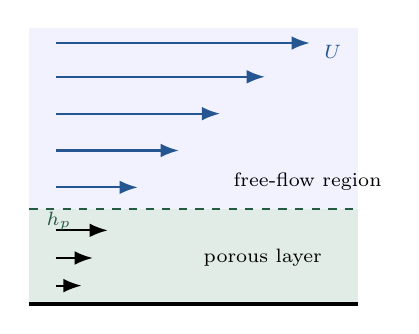
\begin{tikzpicture}[x=0.95cm,y=0.78cm,>=Latex]
  \fill[plankgreen!15] (0,0) rectangle (4.4,1.55);
  \fill[blue!5] (0,1.55) rectangle (4.4,4.5);
  \draw[very thick] (0,0)--(4.4,0);
  \draw[thick,dashed,plankgreen!70!black] (0,1.55)--(4.4,1.55);
  \draw[->,thick] (0.35,0.3)--(0.7,0.3);
  \draw[->,thick] (0.35,0.75)--(0.85,0.75);
  \draw[->,thick] (0.35,1.2)--(1.05,1.2);
  \draw[->,thick,plankblue] (0.35,1.9)--(1.45,1.9);
  \draw[->,thick,plankblue] (0.35,2.5)--(2.0,2.5);
  \draw[->,thick,plankblue] (0.35,3.1)--(2.55,3.1);
  \draw[->,thick,plankblue] (0.35,3.7)--(3.15,3.7);
  \draw[->,thick,plankblue] (0.35,4.25)--(3.75,4.25);
  \node[anchor=west] at (2.2,0.75){\scriptsize porous layer};
  \node[anchor=west] at (2.6,2.0){\scriptsize free-flow region};
  \node[anchor=west,plankgreen!70!black] at (0.1,1.35){\scriptsize \(h_p\)};
  \node[anchor=east,plankblue] at (4.3,4.1){\scriptsize \(U\)};
\end{tikzpicture}
\source{Code adapted from \texttt{examples/basic\_ex\_2d.py}.}
\end{column}
\end{columns}
\end{frame}

% ----- 12. Flow representation -----
\begin{frame}[fragile]{Read the field representation before moving agents}
\small
\begin{columns}[T,onlytextwidth]
\begin{column}{0.54\textwidth}
\begin{lstlisting}
print(len(env.flow))
print([a.shape for a in env.flow])
print(env.flow_points)
print(env.flow_times)
print(env.L, env.units)
\end{lstlisting}
\begin{block}{Array convention}
\begin{itemize}\itemsep2pt
  \item static: \texttt{(nx, ny[, nz])};
  \item time-dependent: \texttt{(nt, nx, ny[, nz])};
  \item one array for each velocity component;
  \item \texttt{flow\_points[i]} indexes spatial axis \(i\).
\end{itemize}
\end{block}
\end{column}
\begin{column}{0.42\textwidth}
\begin{block}{Interpolation contract}
Planktos uses linear spatial interpolation on a rectilinear grid and cubic splines in time for time-dependent data.
\end{block}
\begin{alertblock}{Preflight checks}
{\footnotesize\begin{itemize}\itemsep0pt
  \item component shapes agree;
  \item coordinate arrays increase and match the axes;
  \item domain boundaries and mesh coordinates align;
  \item \texttt{flow\_times} spans the intended run;
  \item speeds and units are physically plausible.
\end{itemize}}
\end{alertblock}
\end{column}
\end{columns}
\end{frame}

% ----- 13. Hand-built field -----
\begin{frame}[fragile]{Supply a hand-built rectilinear velocity field}
\small
\begin{columns}[T,onlytextwidth]
\begin{column}{0.59\textwidth}
\begin{lstlisting}
import numpy as np
import planktos

x = np.linspace(0, 2, 81)
y = np.linspace(0, 1, 41)
X, Y = np.meshgrid(x, y, indexing="ij")

u = 4*Y*(1-Y)          # streamwise component
v = np.zeros_like(u)

env = planktos.Environment(
    Lx=x[-1], Ly=y[-1], flow=[u, v])
env.flow_points = (x, y)
env.plot_flow()
\end{lstlisting}
\end{column}
\begin{column}{0.37\textwidth}
\footnotesize
\begin{block}{Why \texttt{indexing="ij"}?}
Axis 0 is \(x\), axis 1 is \(y\). This matches the current Planktos storage convention and avoids a silent transpose.
\end{block}
\begin{block}{Time-dependent fields}
Stack snapshots on axis 0 and pass \texttt{flow\_times} to the constructor. The remaining axes stay \((x,y[,z])\).
\end{block}
\begin{alertblock}{Coordinates}
Set \texttt{flow\_points} explicitly when the coordinates are not the constructor's uniform grid.
\end{alertblock}
\end{column}
\end{columns}
\source{Convention cross-checked against current flow-generation and analysis tests.}
\end{frame}

% ----- 14. Add a Swarm -----
\begin{frame}[fragile]{Add a vectorized swarm}
\begin{columns}[T,onlytextwidth]
\begin{column}{0.57\textwidth}
\begin{lstlisting}
# Convenience method: automatically uses env
s = env.add_swarm(
    swarm_size=200,
    init="random", seed=2026,
    name="larvae", color="darkgreen")

# Equivalent explicit construction
s2 = planktos.Swarm(
    swarm_size=50, envir=env,
    init=(0.1, 0.5), seed=7)

print(s.N, s.positions.shape)
print(len(env.swarms))
\end{lstlisting}
\end{column}
\begin{column}{0.39\textwidth}
\begin{block}{State layout}
\begin{itemize}\itemsep4pt
  \item \texttt{positions}: masked \(N\times d\) array;
  \item \texttt{velocities}: \(N\times d\);
  \item \texttt{accelerations}: \(N\times d\);
  \item \texttt{props}: per-agent DataFrame;
  \item \texttt{shared\_props}: shared dictionary.
\end{itemize}
\end{block}
\begin{punchbox}
Vectorization is the design choice: write array operations over agents whenever possible.
\end{punchbox}
\end{column}
\end{columns}
\end{frame}

% ----- 15. Initial conditions -----
\begin{frame}[fragile]{Choose initial positions deliberately}
\footnotesize
\begin{columns}[T,onlytextwidth]
\begin{column}{0.59\textwidth}
\begin{lstlisting}
# Uniform random over the domain
s_random = env.add_swarm(500, init="random", seed=1)

# One shared starting point
s_point = env.add_swarm(100, init=(0.15, 0.50), seed=2)

# Explicit N-by-d array
rng = np.random.default_rng(3)
xy = np.column_stack((
    rng.uniform(0.05, 0.15, 300),
    rng.uniform(0.20, 0.80, 300)))
s_patch = env.add_swarm(init=xy, seed=3)

# Grid, optionally excluding closed mesh interiors
s_grid = env.add_swarm(
    init="grid", grid_dim=(80, 40), testdir="x1")
\end{lstlisting}
\end{column}
\begin{column}{0.37\textwidth}
\begin{block}{Interpretation}
\begin{itemize}\itemsep4pt
  \item \texttt{random}: a uniform domain sample;
  \item point: a release cohort;
  \item \(N\times d\) array: measured or designed initial condition;
  \item \texttt{grid}: transport-map or FTLE seed lattice.
\end{itemize}
\end{block}
\begin{alertblock}{Grid masking}
{\footnotesize\texttt{testdir} is meaningful only when a closed immersed mesh is loaded and the chosen ray direction gives a robust inside/outside test.}
\end{alertblock}
\end{column}
\end{columns}
\end{frame}

% ----- 16. Properties and RNG -----
\begin{frame}[fragile]{Shared properties, individual variation, and seeds}
\begin{columns}[T,onlytextwidth]
\begin{column}{0.59\textwidth}
\begin{lstlisting}
import numpy as np

# Same for every agent
s.shared_props["mu"] = np.array([0.0, 0.0])
s.shared_props["cov"] = np.eye(2)*(0.01**2)
s.shared_props["diam"] = 1.0e-3

# One value per agent
rng = np.random.default_rng(2026)
s.props["swim_speed"] = rng.lognormal(
    mean=np.log(0.02), sigma=0.15, size=s.N)

# Uniform access: scalar/array as appropriate
speed = s.get_prop("swim_speed")
diam = s.get_prop("diam")
\end{lstlisting}
\end{column}
\begin{column}{0.37\textwidth}
\begin{block}{The two random streams}
\begin{itemize}\itemsep3pt
  \item \texttt{seed=} initializes \texttt{s.rndState}, used by built-in stochastic motion.
  \item A separate NumPy generator should seed any user-created initial conditions or properties.
\end{itemize}
\end{block}
\begin{alertblock}{Covariance units}
The default SDE uses step covariance \(\texttt{cov}\,dt\). Thus \texttt{cov} has units of length\(^2\)/time, not length\(^2\) per step.
\end{alertblock}
\end{column}
\end{columns}
\end{frame}

% ----- 17. Default SDE -----
\begin{frame}{The default model is Euler--Maruyama drift--diffusion}
For each active agent, the default \texttt{apply\_agent\_model} approximates
\[
  d\vect X
  = \left[\vect u(\vect X,t)+\vect\mu\right]dt
    + \boldsymbol\sigma\,d\vect W_t,
  \qquad
  \texttt{cov}=\boldsymbol\sigma\boldsymbol\sigma^{T}=2\boldsymbol D.
\]
One step is
\[
  \vect X^{n+1,*}=\vect X^n+
  \left[\vect u(\vect X^n,t^n)+\vect\mu\right]\Delta t
  +\mathcal N\!\left(\vect 0,\texttt{cov}\,\Delta t\right),
\]
followed by outer-boundary and immersed-mesh handling.

\begin{columns}[T,onlytextwidth]
\begin{column}{0.48\textwidth}
\begin{block}{Deterministic tracer}
For spatial dimension (d), set \texttt{mu = np.zeros(d)} and \texttt{cov = np.zeros((d,d))}; then motion is forward Euler using the local fluid velocity.
\end{block}
\end{column}
\begin{column}{0.48\textwidth}
\begin{alertblock}{Time-step audit}
Check both temporal convergence and collision resolution. A step can be statistically reasonable yet too large to resolve a narrow obstacle.
\end{alertblock}
\end{column}
\end{columns}
\end{frame}

% ----- 18. Advance and history -----
\begin{frame}[fragile]{Advance the swarm and read its histories}
\small
\begin{columns}[T,onlytextwidth]
\begin{column}{0.58\textwidth}
\begin{lstlisting}
import numpy as np

dt = 0.1
for _ in range(round(24.0/dt)):
    s.move(dt, silent=True)

print(env.time)
print(len(env.time_history))
print(len(s.full_pos_history))

# Current diagnostics
mask = np.ma.getmaskarray(s.positions)
active = ~np.all(mask, axis=1)
print(active.sum(), "agents remain active")
print(s.velocities.mean(axis=0))
\end{lstlisting}
\end{column}
\begin{column}{0.38\textwidth}
\begin{block}{What \texttt{move} manages}
\begin{enumerate}\itemsep2pt
  \item calls \texttt{apply\_agent\_model(dt)};
  \item stores prior position/velocity/property state;
  \item estimates velocity and acceleration;
  \item applies boundaries and mesh collisions;
  \item calls \texttt{after\_move(dt)};
  \item advances environment time.
\end{enumerate}
\end{block}
{\scriptsize\hi{History note:} \texttt{full\_pos\_history} and \texttt{full\_vel\_history} return stored history plus the current state without mutating it.}
\end{column}
\end{columns}
\end{frame}

% ----- 19. Multiple swarms -----
\begin{frame}[fragile]{Move multiple swarms on one shared clock}
\begin{columns}[T,onlytextwidth]
\begin{column}{0.56\textwidth}
\begin{lstlisting}
tracers = env.add_swarm(
    500, seed=10, name="tracers", color="navy")
swimmers = env.add_swarm(
    500, seed=11, name="swimmers", color="orange")
swimmers.shared_props["mu"] = np.array([0.02, 0.0])

for _ in range(400):
    env.move_swarms(
        dt=0.05,
        ib_collisions="sliding",
        silent=True)
\end{lstlisting}
\end{column}
\begin{column}{0.40\textwidth}
\centering
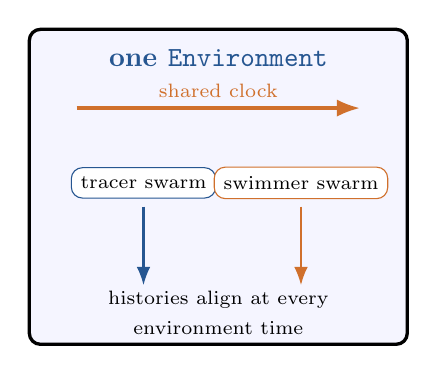
\begin{tikzpicture}[>=Latex]
  \draw[very thick,rounded corners,fill=blue!4] (0,0) rectangle (4.8,4.0);
  \node[font=\bfseries,text=plankblue] at (2.4,3.63){one \texttt{Environment}};
  \draw[->,very thick,plankorange] (0.6,3.0)--(4.2,3.0) node[midway,above]{\scriptsize shared clock};
  \node[draw=plankblue,fill=white,rounded corners] at (1.45,2.05){\scriptsize tracer swarm};
  \node[draw=plankorange,fill=white,rounded corners] at (3.45,2.05){\scriptsize swimmer swarm};
  \draw[->,plankblue,thick] (1.45,1.75)--(1.45,0.75);
  \draw[->,plankorange,thick] (3.45,1.75)--(3.45,0.75);
  \node[align=center] at (2.4,0.40){\scriptsize histories align at every\\[-1pt]\scriptsize environment time};
\end{tikzpicture}
\begin{alertblock}{Avoid double time advancement}
Do not call \texttt{s1.move(dt)} and then \texttt{s2.move(dt)} when both should occupy the same time step. Use \texttt{env.move\_swarms}.
\end{alertblock}
\end{column}
\end{columns}
\end{frame}

% ----- 20. Static plotting -----
\begin{frame}[fragile]{Make an early diagnostic plot}
\begin{columns}[T,onlytextwidth]
\begin{column}{0.52\textwidth}
\begin{lstlisting}
# Current state with velocity arrows
s.plot(
    fluid="quiver",
    dist="density",
    circ_rad=0.08,
    plot_heading=False)

# Closest stored state to t=8.0
s.plot(
    t=8.0,
    filename="snapshot.png",
    fluid="vort",
    save_kwargs={"dpi": 200})
\end{lstlisting}
\begin{block}{2D fluid overlays}
\texttt{fluid="quiver"} shows velocity vectors; \texttt{fluid="vort"} shows scalar vorticity. These overlays are 2D-only.
\end{block}
\end{column}
\begin{column}{0.45\textwidth}
\centering
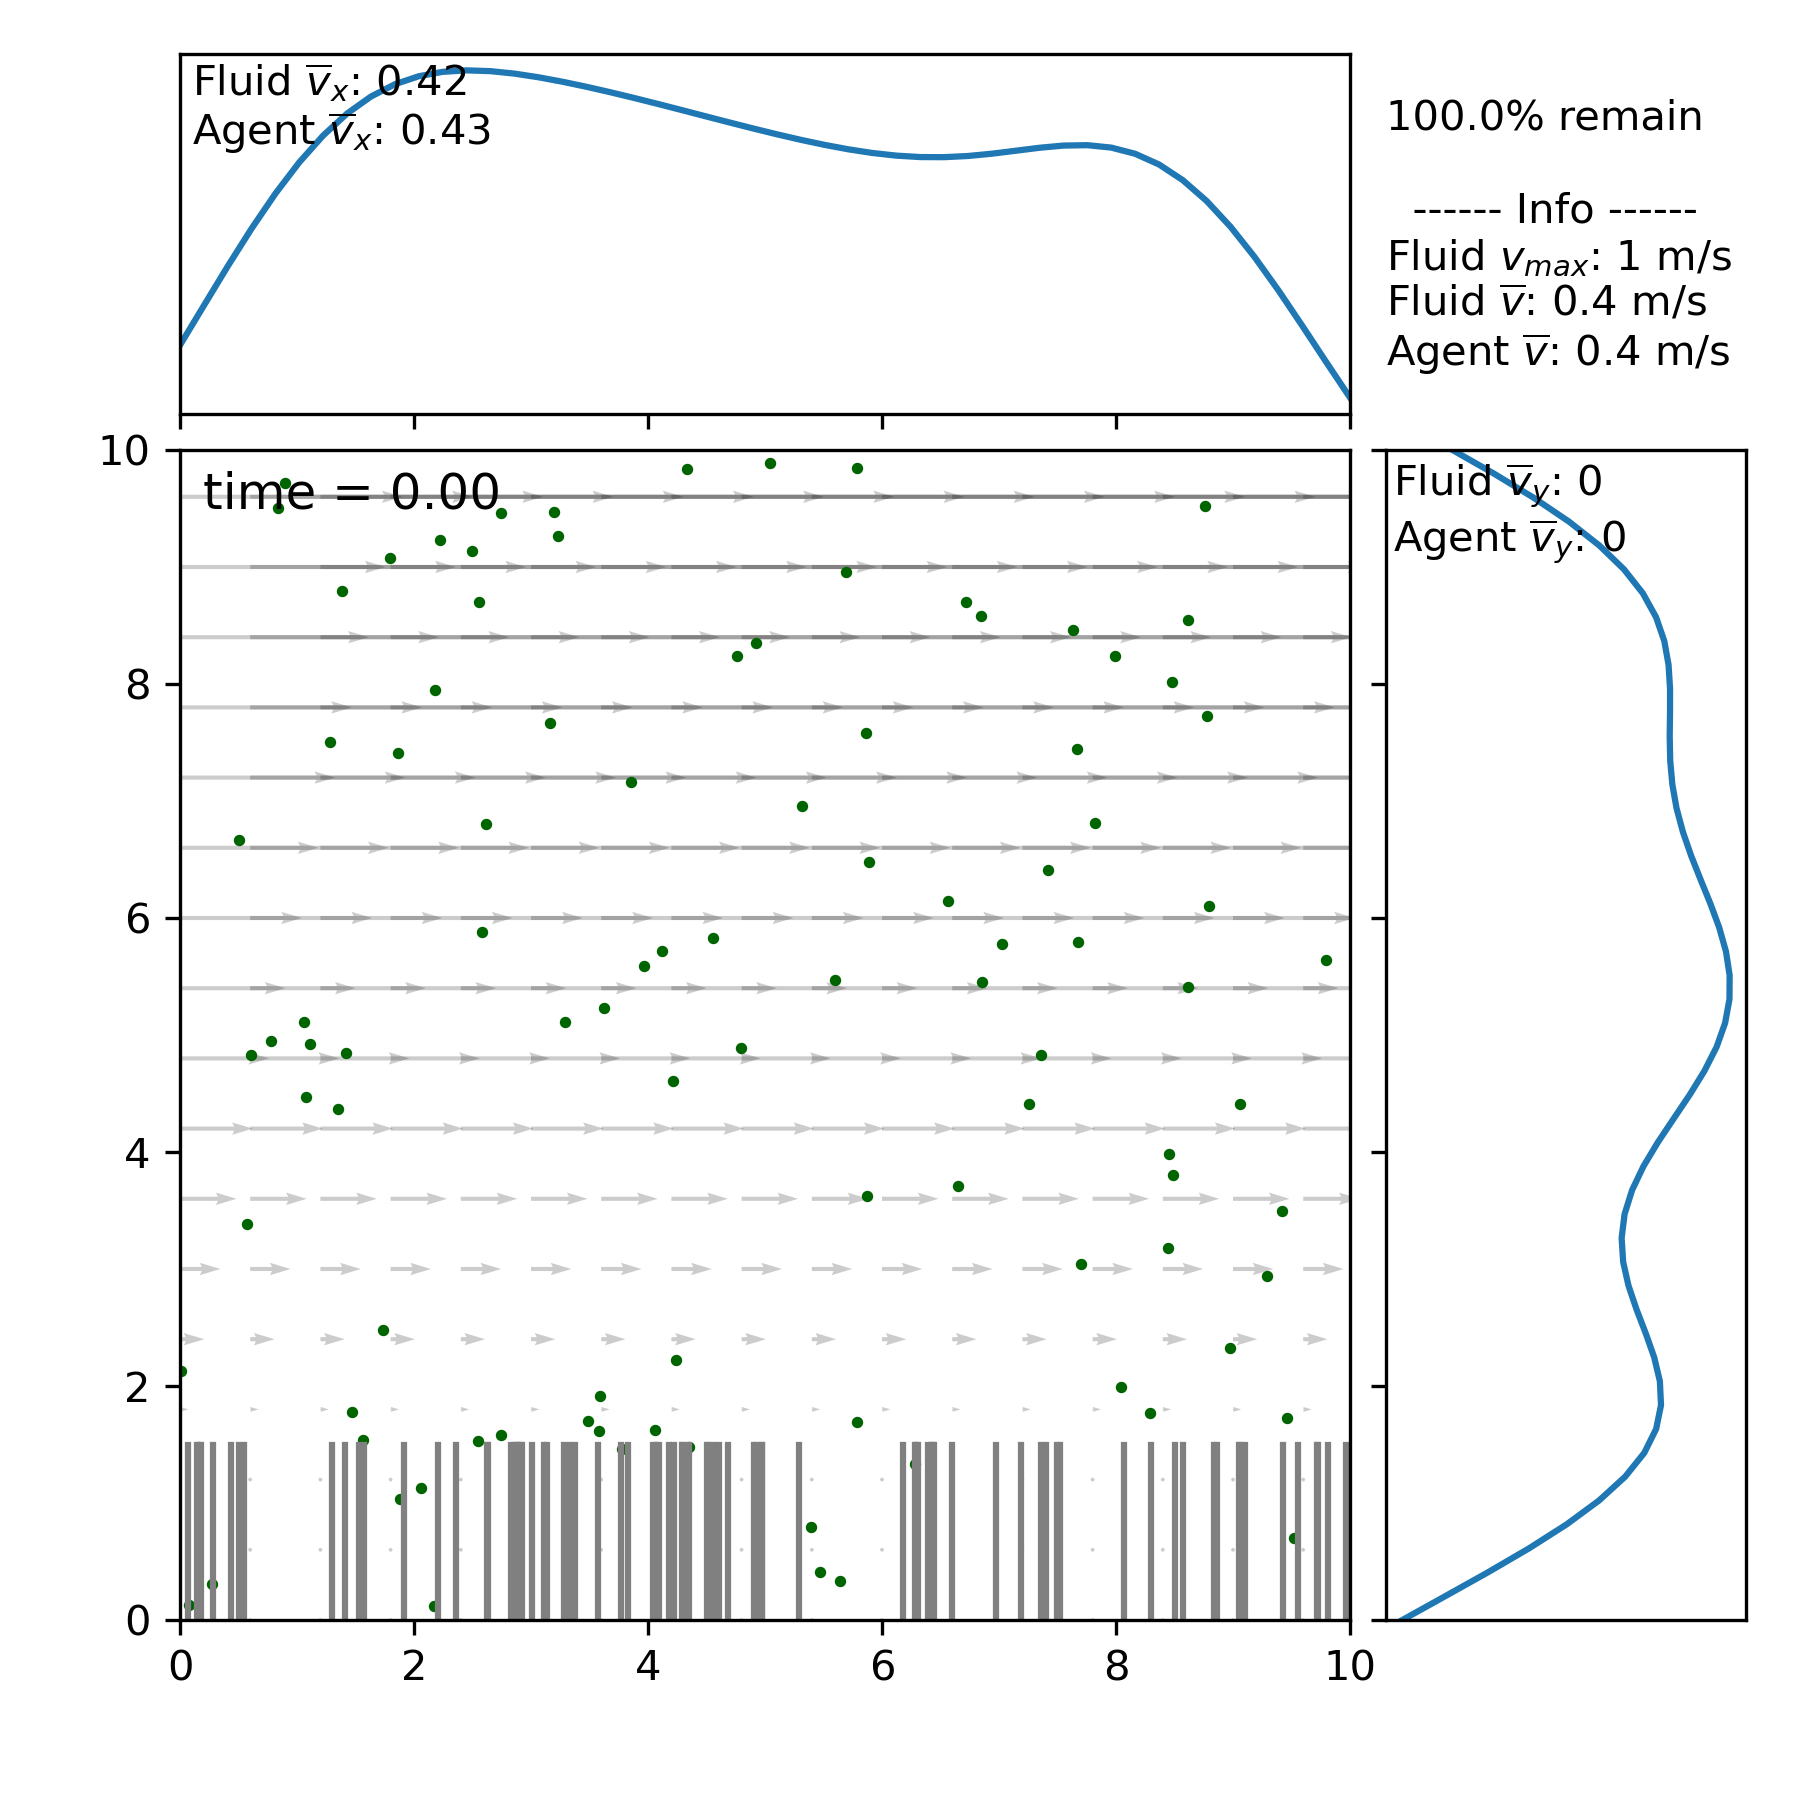
\includegraphics[width=\linewidth,height=0.63\textheight,keepaspectratio]{repo-basic-2d-agents.png}
\source{Not the output of the calls above, but a documentation render of the same example: Planktos documentation image \texttt{docs/\_static/basic\_ex\_2d\_agents.png} (commit \texttt{a1c2128}, GPLv3).}
\end{column}
\end{columns}
\end{frame}

% ----- 21. KDE -----
\begin{frame}[fragile]{KDE turns particles into a distribution diagnostic}
\small
\begin{columns}[T,onlytextwidth]
\begin{column}{0.49\textwidth}
\begin{lstlisting}
# Gaussian KDE with Scott's factor
s.plot(dist="density", fluid="vort")

# Covariance-based width
s.plot(dist="cov", fluid="vort")

# User bandwidth factor or a histogram
s.plot(dist=0.35)
s.plot(dist="hist")
\end{lstlisting}
\begin{itemize}\itemsep0pt
  \item Compare concentration shape, tails, and obstacle wakes.
  \item Report the bandwidth rule with any quantitative comparison.
  \item Check sensitivity to sample size and boundary truncation.
  \item A KDE is a smoothed estimator, not a separately solved concentration field.
\end{itemize}
\end{column}
\begin{column}{0.48\textwidth}
\centering
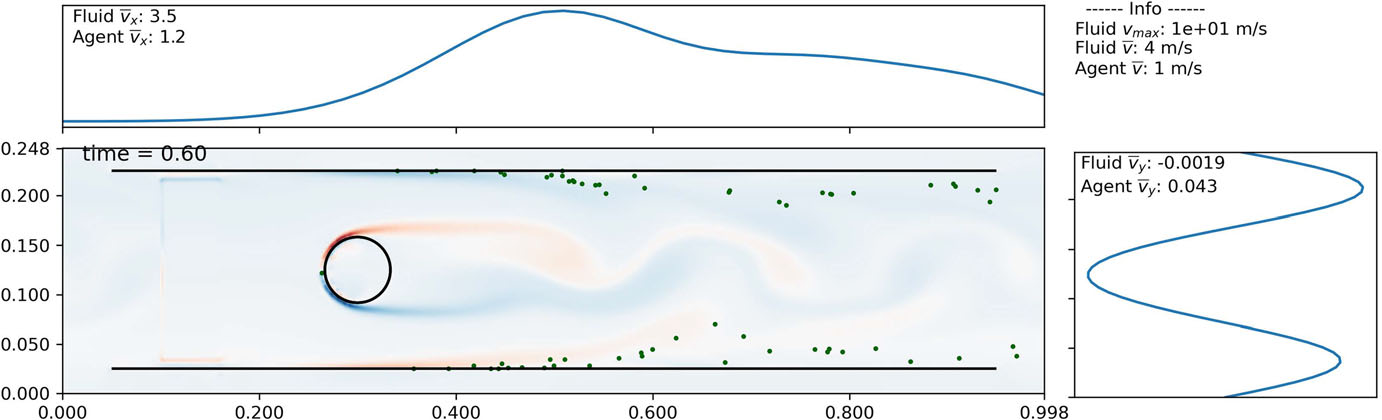
\includegraphics[width=\linewidth,height=0.51\textheight,keepaspectratio]{bmb2022-fig4-ib2d-kde.png}
\source{IB2d cylinder flow, agents, vorticity, and marginal density: Strickland et al. (2022), Fig.~4; educational reproduction.}
\end{column}
\end{columns}
\end{frame}

% ----- 22. Animation and export -----
\begin{frame}[fragile]{Animate selectively; export analysis-ready data}
\small
\begin{columns}[T,onlytextwidth]
\begin{column}{0.60\textwidth}
\begin{lstlisting}
# Use every fifth stored state
frames = range(0, len(s.full_pos_history), 5)
s.plot_all(
    movie_filename="trial_01.mp4",
    frames=frames, fps=10,
    fluid="vort", plot_heading=False)

# Data products
s.save_data("results", "trial_01")
s.save_pos_to_csv("results/trial_01_positions.csv")
s.save_pos_to_vtk("results", "trial_01")
\end{lstlisting}
\end{column}
\begin{column}{0.36\textwidth}
\begin{block}{Choose the product by use}
\begin{itemize}\itemsep1pt
  \item \texttt{save\_data}: position history plus current kinematics and properties;
  \item CSV: portable position history;
  \item VTK: ParaView/VisIt workflow;
  \item MP4: communication, not raw data.
\end{itemize}
\end{block}
\begin{alertblock}{Cost control}
{\footnotesize Use \texttt{frames} for temporal subsampling and \texttt{downsamp} for display-only agent subsampling. Statistics still use the full population.}
\end{alertblock}
\end{column}
\end{columns}
\vspace{-2pt}
\source{Calls match current \texttt{Swarm.plot\_all} and save-method signatures.}
\end{frame}

% ----- 23. Subclass contract -----
\begin{frame}[fragile]{Custom behavior: override one hook, not the harness}
\begin{columns}[T,onlytextwidth]
\begin{column}{0.53\textwidth}
\begin{lstlisting}
class MySwarm(planktos.Swarm):
    def apply_agent_model(self, dt):
        # Compute proposed N-by-d positions.
        new_positions = ...
        return new_positions
\end{lstlisting}
\begin{block}{Contract}
\begin{itemize}\itemsep3pt
  \item keep the signature \texttt{(self, dt)};
  \item return an \(N\times d\) array;
  \item do not assign \texttt{positions}, \texttt{velocities}, or \texttt{accelerations};
  \item let \texttt{move} record history and apply collisions.
\end{itemize}
\end{block}
\end{column}
\begin{column}{0.43\textwidth}
\begin{alertblock}{Current versus historical API}
The 2022 paper describes a historical override named \texttt{get\_positions}. The current v1.0.3 repository and examples use \texttt{apply\_agent\_model(self, dt)}.
\end{alertblock}
\begin{punchbox}
\raggedright
Use \texttt{after\_move(dt)} for state changes based on the accepted, collision-corrected endpoint.
\end{punchbox}
\end{column}
\end{columns}
\source{Current contract: \texttt{planktos/\_swarm.py} and \texttt{examples/ex\_agent\_behavior.py}.}
\end{frame}

% ----- 24. Custom deterministic behavior -----
\begin{frame}[fragile]{Example: fluid advection plus directed swimming}
\begin{columns}[T,onlytextwidth]
\begin{column}{0.61\textwidth}
\begin{lstlisting}
import numpy as np
import planktos

class TargetSwarm(planktos.Swarm):
    def apply_agent_model(self, dt):
        target = np.array([1.8, 0.5])
        direction = target - self.positions
        norm = np.linalg.norm(direction, axis=1)[:, None]
        direction = direction/np.maximum(norm, 1.0e-12)

        speed = self.get_prop("swim_speed")[:, None]
        velocity = self.get_fluid_drift() + speed*direction
        return self.positions + velocity*dt
\end{lstlisting}
\end{column}
\begin{column}{0.35\textwidth}
\begin{block}{Useful field queries}
{\scriptsize
\begin{itemize}\itemsep2pt
  \item \texttt{get\_fluid\_drift()};
  \item \texttt{get\_dudt()};
  \item \texttt{get\_fluid\_mag\_gradient()};
  \item \texttt{get\_DuDt()}.
\end{itemize}}
\end{block}
\begin{alertblock}{Numerical hygiene}
Guard normalizations, preserve masks, and call expensive interpolants once per time step rather than once per agent.
\end{alertblock}
\end{column}
\end{columns}
\source{Pattern adapted from \texttt{examples/ex\_agent\_behavior.py}.}
\end{frame}

% ----- 25. ODE motion -----
\begin{frame}[fragile]{Deterministic ODE motion with the RK45 wrapper}
\begin{columns}[T,onlytextwidth]
\begin{column}{0.60\textwidth}
\begin{lstlisting}
import planktos
from planktos import motion

class AccurateTracer(planktos.Swarm):
    def apply_agent_model(self, dt):
        ode = motion.tracer_particles(
            self, incl_dvdt=False)
        t0 = self.envir.time
        # positions is a masked array; strip masked
        # (exited) rows before RK45, as calculate_FTLE does
        return motion.RK45(
            ode, t0, self.positions.copy(), t0 + dt,
            rtol=1.0e-6, atol=1.0e-9)
\end{lstlisting}
\end{column}
\begin{column}{0.36\textwidth}
\begin{block}{Current solver contract}
\texttt{motion.RK45} wraps SciPy \texttt{solve\_ivp}; the right-hand side has signature \texttt{fun(t, x)} and returns the same 2D shape as \texttt{x}.
\end{block}
\begin{alertblock}{Two time scales}
The internal ODE solver adapts substeps, but Planktos applies boundary and mesh collision handling only after the outer \texttt{move(dt)} proposal.
\end{alertblock}
\end{column}
\end{columns}
\end{frame}

% ----- 26. SDE with ODE drift -----
\begin{frame}[fragile]{Combine an ODE drift with stochastic motion}
\begin{columns}[T,onlytextwidth]
\begin{column}{0.60\textwidth}
\begin{lstlisting}
import numpy as np
import planktos
from planktos import motion

def social_bias(pos):
    return 0.1*(pos.mean(axis=0) - pos)

def behavior_ode(swarm):
    def rhs(t, x):
        N = x.shape[0]//2
        vel = swarm.get_fluid_drift(t, x[:N])
        vel += social_bias(x[:N])
        return np.concatenate((
            vel, np.zeros((N, x.shape[1]))))
    return rhs

class SocialSwarm(planktos.Swarm):
    def apply_agent_model(self, dt):
        return motion.Euler_brownian_motion(
            self, dt, ode=behavior_ode(self))
\end{lstlisting}
\end{column}
\begin{column}{0.36\textwidth}
\begin{block}{State convention}
An ODE passed to \texttt{Euler\_brownian\_motion} receives \(2N\times d\): positions followed by velocities. It returns their time derivatives in the same layout.
\end{block}
\begin{alertblock}{Fluid drift is explicit}
When an \texttt{ode} is supplied, include fluid interaction in that ODE if it is part of the model; it is not added automatically there.
\end{alertblock}
\end{column}
\end{columns}
\source{Adapted from \texttt{examples/ex\_ode\_gen.py}.}
\end{frame}

% ----- 27. Inertial particles -----
\begin{frame}[fragile]{Built-in inertial-particle dynamics}
\footnotesize
{\scriptsize\textcolor{red!75!black}{\textbf{Set \(\rho\), \(\mu\), \(\nu\) in the constructor:}} the property setters in v1.0.3 compute \(\mu=\nu/\rho\) (bug, reported upstream).}
\begin{columns}[T,onlytextwidth]
\begin{column}{0.58\textwidth}
\begin{lstlisting}[basicstyle=\ttfamily\fontsize{6.3}{7.0}\selectfont]
import numpy as np
import planktos
from planktos import motion

zero = np.zeros((3, 3))
env = planktos.Environment(
    Lx=1, Ly=1, rho=1000, nu=1e-6,
    char_L=0.01, U=0.1,
    flow=[zero, zero.copy()])

class InertialSwarm(planktos.Swarm):
    def apply_agent_model(self, dt):
        ode = motion.inertial_particles(self)
        # positions is a masked array; strip masked
        # (exited) rows before RK45, as calculate_FTLE does
        # NB: move() overwrites velocities with
        # (x_new-x_old)/dt; persist velocity in props
        # for a true second-order model
        state = np.ma.concatenate(
            (self.positions, self.velocities))
        out = motion.RK45(
            ode, self.envir.time, state,
            self.envir.time + dt)
        return out[:self.N]

s = InertialSwarm(envir=env, seed=4)
s.shared_props.update({"R": 2/3, "diam": 1e-4})
\end{lstlisting}
\end{column}
\begin{column}{0.38\textwidth}
\begin{block}{Required environment data}
A velocity field (explicit zeros are valid), \texttt{char\_L}, \texttt{U}, \texttt{nu}, and gravity; fluid density unless \texttt{R} is supplied.
\end{block}
\begin{block}{Required particle data}
Density ratio \texttt{R} (or particle \texttt{rho}) and diameter \texttt{diam}.
\end{block}
\begin{alertblock}{Model regime}
The implementation is the linearized Maxey--Riley form documented for \(R/\mathrm{St}\gg1\); verify that approximation for the particles and flow under study. Here, the displayed parameters give \(R/\mathrm{St}\approx120\).
\end{alertblock}
\end{column}
\end{columns}
\end{frame}

% ----- 28. Collision modes -----
\begin{frame}{Immersed-mesh collision modes}
\small
\begin{columns}[T,onlytextwidth]
\begin{column}{0.48\textwidth}
\scriptsize
\begin{tabular}{@{}p{0.24\linewidth}p{0.67\linewidth}@{}}
\toprule
\textbf{Mode} & \textbf{Proposed step after a mesh hit} \\
\midrule
\texttt{sliding} & Project motion along the boundary, recursively using remaining displacement. \\
\texttt{sticky} & Stop at the first point of intersection for that time step. \\
\texttt{None} & Ignore immersed meshes. \\
\texttt{'default'} & Use the Swarm's \texttt{ib\_condition} (default \texttt{'sliding'}). \\
\bottomrule
\end{tabular}
\vspace{0.5em}
Set a swarm default with \texttt{ib\_condition}; override per step with
\[
 \texttt{s.move(dt, ib\_collisions="sticky")}.
\]
\texttt{s.ib\_collision\_idx} is a per-agent array of the last-step element index hit, \(-1\) if none.
\end{column}
\begin{column}{0.49\textwidth}
\centering
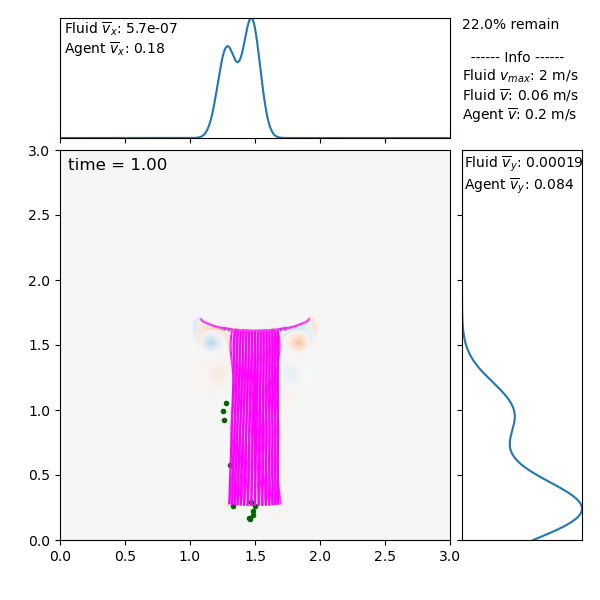
\includegraphics[width=\linewidth,height=0.43\textheight,keepaspectratio]{repo-moving-boundary-sticky.png}
\source{Sticky agents and a moving IB2d boundary; Planktos documentation image \texttt{docs/\_static/ib2d\_mvbnd\_sticky.png} (commit \texttt{a1c2128}, GPLv3).}
\begin{alertblock}{Geometry restriction}
{\footnotesize Avoid immersed structures that intersect periodic box boundaries; that interaction is not implemented in the current API.}
\end{alertblock}
\end{column}
\end{columns}
\end{frame}

% ----- 29. Stateful capture -----
\begin{frame}[fragile]{Make ``captured'' a persistent biological state}
\small
\begin{columns}[T,onlytextwidth]
\begin{column}{0.58\textwidth}
\begin{lstlisting}
import numpy as np
from planktos import motion

class CaptureSwarm(planktos.Swarm):
    def apply_agent_model(self, dt):
        proposed = motion.Euler_brownian_motion(self, dt)
        held = self.get_prop("captured")[:, None]
        return np.ma.where(held, self.positions, proposed)

    def after_move(self, dt):
        hit = self.ib_collision_idx >= 0
        self.props.loc[hit, "captured"] = True
        self.props.loc[hit, "color"] = "gold"

s = CaptureSwarm(
    envir=env, ib_condition="sticky",
    store_prop_history=True)
s.props["captured"] = np.zeros(s.N, dtype=bool)
s.props["color"] = np.full(s.N, s.shared_props["color"])
\end{lstlisting}
\end{column}
\begin{column}{0.38\textwidth}
\centering

\includegraphics[width=\linewidth,height=0.27\textheight,keepaspectratio]{jeb2023-fig6a-polyp-array.png}
\source{Cylinder and polyp geometry: Hamlet et al. (2023), Fig.~6a, CC BY 4.0.}
\begin{block}{Why both hooks?}
\texttt{after\_move} records new contacts after collision correction. \texttt{apply\_agent\_model} prevents previously captured agents from leaving on later steps.
\end{block}
\end{column}
\end{columns}
\source{Pattern adapted from \texttt{examples/ex\_sticky\_seafan\_3d.py}.}
\end{frame}

% ----- 30. IB2d import -----
\begin{frame}[fragile]{Import an IB2d velocity field and 2D mesh}
\small
\begin{columns}[T,onlytextwidth]
\begin{column}{0.59\textwidth}
\begin{lstlisting}
env = planktos.Environment()

# From the repository root, first follow
# examples/ib2d_data/README.txt to download the data.
env.read_IB2d_fluid_data(
    "examples/ib2d_data",
    dt=5.0e-5, print_dump=1000)

env.read_IB2d_mesh_data(
    "examples/ib2d_data/channel.vertex",
    method="proximity")

env.plot_envir()
s = planktos.Swarm(
    envir=env, init=(0.1*env.L[0], 0.5*env.L[1]),
    seed=1)
\end{lstlisting}
\end{column}
\begin{column}{0.37\textwidth}
\begin{block}{Time mapping}
\footnotesize
Successive printed flow snapshots are separated by
\[
  \Delta t_{\mathrm{data}}
  =\texttt{dt}\times\texttt{print\_dump}=0.05.
\]
\end{block}
\begin{block}{Mesh association}
\footnotesize
\texttt{proximity} connects nearby vertices. It can infer resolution from loaded flow or accept \texttt{res=} explicitly.
\end{block}
{\footnotesize\textcolor{red!75!black}{\textbf{Inspect connectivity.}} Crossing segments without a shared vertex can create collision leaks. Always call \texttt{plot\_envir()}.}
\end{column}
\end{columns}
\source{Adapted from \texttt{examples/ex\_ib2d\_ibmesh.py}; the external dataset is linked from \texttt{examples/ib2d\_data/README.txt}.}
\end{frame}

% ----- 31. Other imports -----
\begin{frame}[fragile]{Import matrix: CFD fields and 3D geometry}
\scriptsize
\begin{tabular}{@{}>{\raggedright\arraybackslash}p{0.18\linewidth}>{\raggedright\arraybackslash}p{0.47\linewidth}>{\raggedright\arraybackslash}p{0.28\linewidth}@{}}
\toprule
\textbf{Source} & \textbf{Current call pattern} & \textbf{Audit item} \\
\midrule
IBAMR 3D VTK & \texttt{env.read\_IBAMR3d\_vtk\_data(path, d\_start=0, d\_finish=None, vel\_conv=None, grid\_conv=None)} & dump range; spatial and velocity conversions \\
\addlinespace
COMSOL VTU & \texttt{env.read\_comsol\_vtu\_data(file, vel\_conv=None, grid\_conv=None)} & cell-centered versus nodal grid; units \\
\addlinespace
NetCDF & \texttt{env.load\_NetCDF(file)} then \texttt{env.read\_NetCDF\_flow("u","v", time\_name="time", dim\_reorder=...)} & variable names, dimension order, component axis, calendar/time units \\
\addlinespace
STL mesh & \texttt{env.read\_stl\_mesh\_data(file, unit\_conv=None)} & mesh and flow share the same coordinate frame \\
\addlinespace
IB2d mesh & \texttt{env.read\_IB2d\_mesh\_data(file, method="adjacent"|"proximity"|"hull")} & breaks/additional edges; closed geometry \\
\bottomrule
\end{tabular}

\vspace{0.55em}
\begin{punchbox}
\centering
The loader may reset \texttt{env.L} to match the data. Read back \texttt{L}, \texttt{flow\_points}, \texttt{flow\_times}, \texttt{fluid\_domain\_LLC}, and units after every import.
\end{punchbox}
\source{Signatures audited against \texttt{planktos/\_environment.py}, v1.0.3.}
\end{frame}

% ----- 32. Mesh and unit QA -----
\begin{frame}[fragile]{Align flow, mesh, and physical units before release}
\begin{columns}[T,onlytextwidth]
\begin{column}{0.54\textwidth}
\begin{lstlisting}
# For appropriate cell-centered COMSOL data,
# regrid immediately after the flow import.
# Match these flags to the data's actual BCs;
# this example treats all axes as nonperiodic.
env.center_cell_regrid(
    periodic_dim=(False, False, False))

# Only then load the immersed geometry.
env.read_stl_mesh_data("geometry.stl")

print("domain:", env.L, env.units)
print("flow origin:", env.fluid_domain_LLC)
print("flow axes:", [p[[0, -1]] for p in env.flow_points])
print("mesh shape:", None if env.ibmesh is None
      else env.ibmesh.shape)

env.plot_envir()
env.plot_flow()
\end{lstlisting}
\end{column}
\begin{column}{0.42\textwidth}
\begin{block}{One consistent conversion ledger}
Record conversions for length, velocity, time, density, viscosity, gravity, particle diameter, and mesh coordinates. Prefer converting on import with \texttt{vel\_conv}, \texttt{grid\_conv}, or \texttt{unit\_conv}.
\end{block}
\begin{alertblock}{Visual mesh audit}
Look for crossing edges, missing closure, duplicated surfaces, mesh outside the flow domain, and unintended contact with a periodic face.
\end{alertblock}
\end{column}
\end{columns}
\end{frame}

% ----- 33. FTLE -----
\begin{frame}[fragile]{FTLE reveals finite-time stretching of a motion model}
\small
\begin{columns}[T,onlytextwidth]
\begin{column}{0.49\textwidth}
Let \(\tau=T-t_0>0\). For the flow map \(\vect\Phi_{t_0}^{T}\), the largest forward-time exponent is
\[
  \sigma_{t_0}^{\tau}(\vect x_0)
  =\frac{1}{\tau}\log\sqrt{\lambda_{\max}\!\left[(D\vect\Phi)^T D\vect\Phi\right]}.
\]
\begin{lstlisting}
env.calculate_FTLE(
    grid_dim=(512, 128),
    t0=0, T=0.1, dt=0.001)
env.plot_2D_FTLE()

# Backward from physical time 0.1 to 0.0:
# current API uses T as the forward pseudo-time endpoint.
env.calculate_FTLE(
    (512, 128), t0=0.1, T=0.2,
    dt=0.001, backward=True)
\end{lstlisting}
\vspace{-2pt}
\source{Calls adapted from \texttt{examples/ex\_produce\_ftle\_2d.py}.}
\end{column}
\begin{column}{0.48\textwidth}
\centering
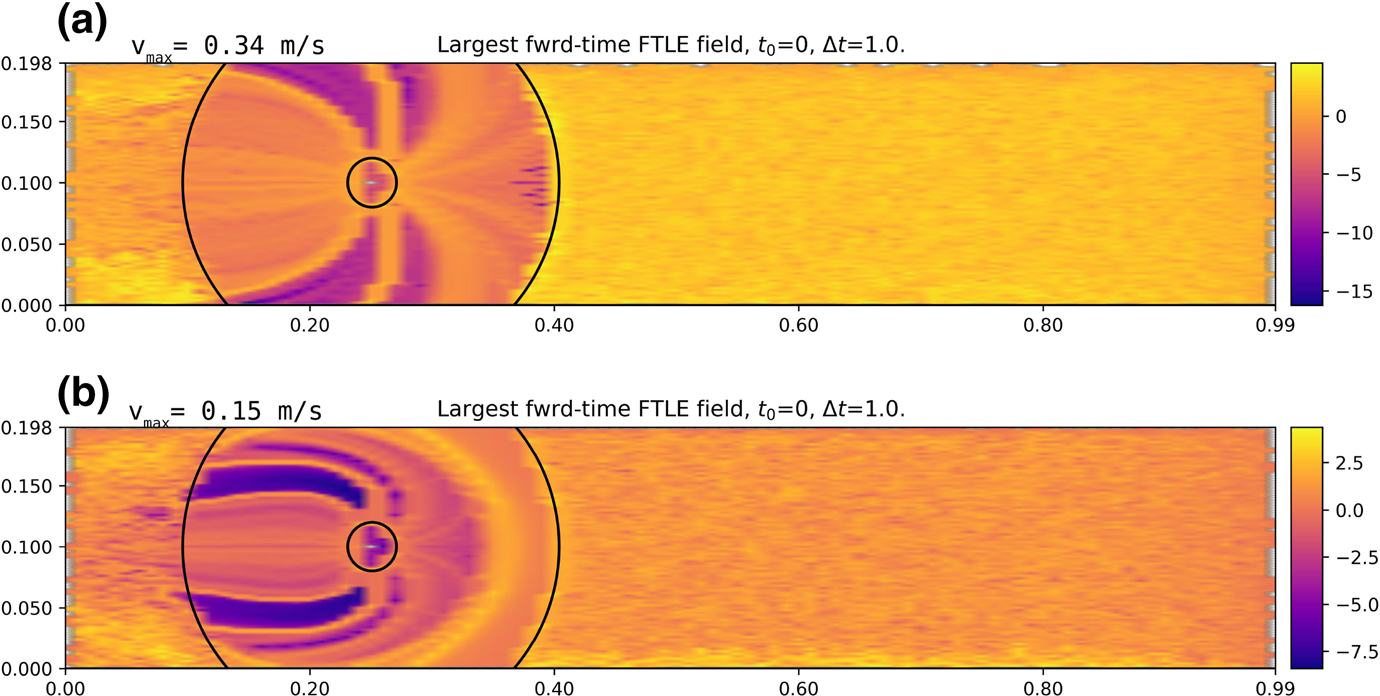
\includegraphics[width=\linewidth,height=0.32\textheight,keepaspectratio]{bmb2022-fig5-ftle.png}
\source{Agent-based forward-time FTLE comparison: Strickland et al. (2022), Fig.~5; educational reproduction.}
\begin{alertblock}{Two API distinctions}
{\scriptsize\begin{itemize}\itemsep0pt
  \item The current call requires \texttt{T > t0}; the elapsed interval is \texttt{T-t0}. With \texttt{backward=True}, physical time ends at \texttt{2*t0-T}.
  \item \texttt{FTLE\_smallest} is a forward-map contraction exponent, not backward-time FTLE.
\end{itemize}}
\end{alertblock}
\end{column}
\end{columns}
\end{frame}

% ----- 34. FTLE validity -----
\begin{frame}{When an agent-based FTLE field is meaningful}
\footnotesize
\begin{columns}[T,onlytextwidth]
\begin{column}{0.56\textwidth}
The \texttt{swrm=} route is appropriate when the seeded agents define one reproducible finite-time map:
\begin{itemize}\itemsep4pt
  \item the motion rule is deterministic;
  \item agents use the same rule and parameter set;
  \item each trajectory acts independently of the other seeded agents;
  \item the map is resolved well enough in time and on the initial-condition grid.
\end{itemize}
\begin{alertblock}{Not an ordinary FTLE map}
Stochastic realizations or social rules that depend on the seeded population do not define a single deterministic particle map. Use ensemble dispersion, encounter, or density diagnostics instead.
\source{Qualification follows Strickland et al. (2022), Sections 2.1 and 4.2.}
\end{alertblock}
\end{column}
\begin{column}{0.40\textwidth}
\centering
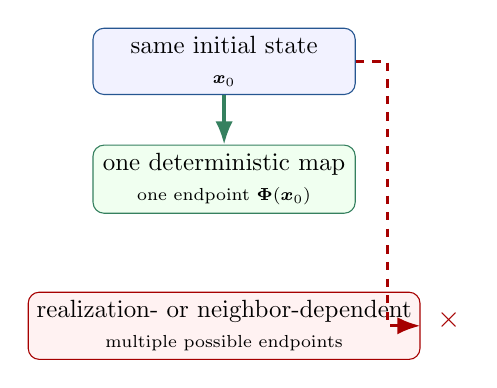
\begin{tikzpicture}[>=Latex,node distance=7mm,scale=0.90,transform shape]
  \node[draw=plankblue,rounded corners,fill=blue!5,align=center,minimum width=3.7cm,minimum height=0.9cm] (x0) {same initial state\\\scriptsize \(\vect x_0\)};
  \node[draw=plankgreen,rounded corners,fill=green!6,align=center,minimum width=3.7cm,minimum height=0.9cm,below=of x0] (one) {one deterministic map\\\scriptsize one endpoint \(\vect\Phi(\vect x_0)\)};
  \draw[->,very thick,plankgreen] (x0)--(one);
  \node[draw=red!65!black,rounded corners,fill=red!5,align=center,minimum width=3.7cm,minimum height=0.9cm,below=11mm of one] (many) {realization- or neighbor-dependent\\\scriptsize multiple possible endpoints};
  \draw[->,very thick,red!65!black,dashed] (x0.east) -- ++(0.45,0) |- (many.east);
  \node[red!65!black,font=\bfseries\large] at ([xshift=4mm,yshift=-4mm]many.north east) {\(\times\)};
\end{tikzpicture}
\vspace{0.4em}
\begin{punchbox}
\centering
FTLE is a property of the chosen finite-time map, not of ``complex-looking'' trajectories in general.
\end{punchbox}
\end{column}
\end{columns}
\end{frame}

% ----- 35. Capstone setup -----
\begin{frame}[fragile]{Capstone: Vicsek agents around an immersed cylinder}
\small
\begin{columns}[T,onlytextwidth]
\begin{column}{0.56\textwidth}
\begin{lstlisting}
import numpy as np
import planktos

env = planktos.Environment(
    Lx=1, Ly=0.25,
    x_bndry="periodic",
    y_bndry="periodic")
env.read_IB2d_mesh_data(
    "examples/vicsek_mesh/channel.vertex",
    method="proximity", res=0.001953125)

rng = np.random.default_rng(2026)
N = 500
IC = np.empty((N, 2))
IC[:, 0] = rng.uniform(0.075, 0.125, N)
IC[:, 1] = rng.uniform(0.050, 0.200, N)
\end{lstlisting}
\end{column}
\begin{column}{0.40\textwidth}
\centering
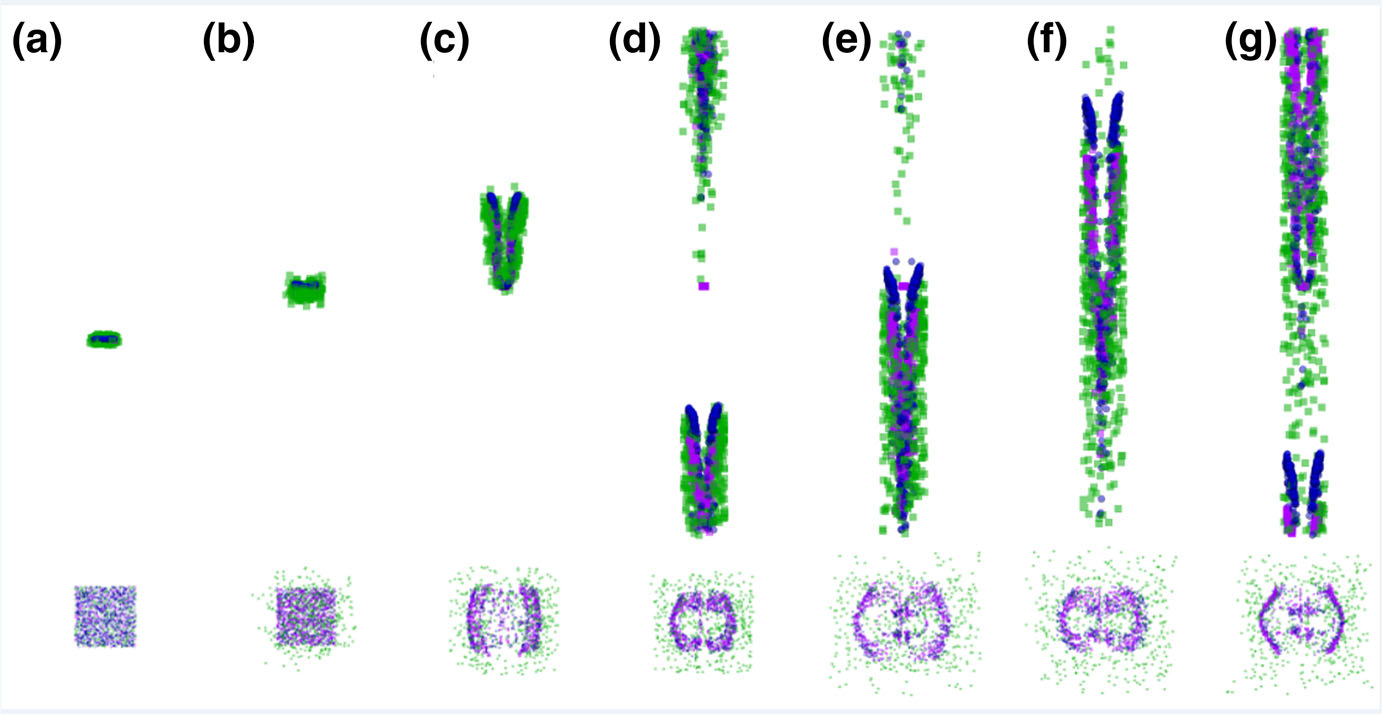
\includegraphics[width=\linewidth,height=0.50\textheight,keepaspectratio]{bmb2022-fig9-vicsek.png}
\source{Motivating 3D result: Strickland et al. (2022), Fig.~9; educational reproduction.}
\begin{block}{Null versus flow experiment}
The repository example runs without the large external flow dataset. Load matching IB2d flow to ask how alignment survives an unsteady wake.
\end{block}
\end{column}
\end{columns}
\source{Setup: current \texttt{examples/ex\_vicsek\_model\_2d.py}; separate NumPy seed added.}
\end{frame}

% ----- 36. Capstone model -----
\begin{frame}[fragile]{Capstone: implement alignment with periodic distances}
\small
\begin{columns}[T,onlytextwidth]
\begin{column}{0.66\textwidth}
\begin{lstlisting}
class Vicsek(planktos.Swarm):
    def __init__(self, *args, **kwargs):
        super().__init__(*args, **kwargs)
        self.shared_props.update(v=0.02, nu=0.5, r=0.1)
        angle = self.get_prop("nu") \
              * (self.rndState.random(self.N)-0.5)
        self.velocities += self.get_prop("v") \
              * np.column_stack((np.cos(angle), np.sin(angle)))

    def apply_agent_model(self, dt):
        theta = np.empty(self.N)
        L = np.asarray(self.envir.L)
        for i, origin in enumerate(self.positions):
            delta = (self.positions-origin + L/2) % L - L/2
            near = np.linalg.norm(delta, axis=1) < self.get_prop("r")
            theta[i] = np.arctan2(
                self.velocities[near, 1].mean(),
                self.velocities[near, 0].mean())
        theta += self.get_prop("nu")*(self.rndState.random(self.N)-0.5)
        active = self.get_prop("v")*np.column_stack((np.cos(theta), np.sin(theta)))
        return self.positions + (active + self.get_fluid_drift())*dt
\end{lstlisting}
\end{column}
\begin{column}{0.30\textwidth}
\begin{block}{Three model ingredients}
\begin{enumerate}\itemsep1pt
  \item average neighbor velocity vectors within radius \texttt{r};
  \item add angular noise of width \texttt{nu};
  \item add self-propulsion speed \texttt{v} and local fluid drift.
\end{enumerate}
\end{block}
\begin{alertblock}{Periodic metric}
{\scriptsize The minimum-image displacement is essential: agents near opposite faces can still be neighbors. Note that the minimum-image wrap assumes periodic boundaries in both axes.}
\end{alertblock}
\end{column}
\end{columns}
\source{Condensed from the current repository Vicsek example; parameter names and hook are unchanged.}
\end{frame}

% ----- 37. Run and validate -----
\begin{frame}[fragile]{Run the capstone, then make the result reproducible}
\footnotesize
\begin{columns}[T,onlytextwidth]
\begin{column}{0.55\textwidth}
\begin{lstlisting}
s = Vicsek(
    swarm_size=N, envir=env, init=IC, seed=2026)

collision_events = 0
for _ in range(72):       # 18 s at dt=0.25 s
    s.move(0.25, silent=True)
    collision_events += np.count_nonzero(
        s.ib_collision_idx >= 0)

print("agent-step collisions:", collision_events)

s.plot_all(
    movie_filename="vicsek_null.mp4",
    fps=4, fluid="vort")
\end{lstlisting}
\begin{block}{Capstone comparisons}
{\footnotesize Repeat with a passive swarm, multiple \texttt{nu}/\texttt{r} values, and at least two smaller \(dt\). Compare polarization, retention, agent-step collisions, and downstream spread.}
\end{block}
\end{column}
\begin{column}{0.41\textwidth}
\begin{block}{Save with every result}
{\scriptsize\begin{itemize}\itemsep0pt
  \item Planktos version/commit and Python/package environment;
  \item flow and mesh provenance plus checksums;
  \item both random seeds and all model parameters;
  \item time step, duration, collision mode, and active-agent count;
  \item code, raw histories, and plotting settings.
\end{itemize}}
\end{block}
\begin{alertblock}{Failure-state diagnostic}
{\scriptsize If a collision step fails, current Planktos marks \texttt{env.time=None}. Inspect the partial state; then restore consistently from histories or restart from a checkpoint.}
\end{alertblock}
\end{column}
\end{columns}
\end{frame}

% ----- 38. Resources -----
\begin{frame}{Resources and source trail}
\begin{columns}[T,onlytextwidth]
\begin{column}{0.55\textwidth}
\begin{block}{Start with the current software}
\begin{itemize}\itemsep4pt
  \item \href{https://github.com/mountaindust/Planktos}{Planktos repository and README};
  \item repository \texttt{docs/} and runnable \texttt{examples/};
  \item \texttt{examples/ib2d\_data/README.txt} for the external IB2d dataset;
  \item this tutorial was audited against v1.0.3, commit \texttt{a1c2128} (2026-08-19).
\end{itemize}
\end{block}
\begin{punchbox}
\centering
Record the exact software commit with every scientific result: current interfaces can differ from those shown in the 2022 paper.
\end{punchbox}
\end{column}
\begin{column}{0.41\textwidth}
\begin{block}{Primary scientific sources}
\small
\href{https://doi.org/10.1007/s11538-022-01027-1}{Strickland et al. (2022), \emph{Bulletin of Mathematical Biology} 84:72}\\[8pt]
Software architecture, agent models, collision handling, visualization, FTLE, and examples.\\[10pt]
\href{https://doi.org/10.1242/jeb.244520}{Hamlet et al. (2023), \emph{Journal of Experimental Biology} 226, jeb244520}\\[8pt]
Gorgonian multiscale flow and capture application; article and reproduced figures are CC BY 4.0.
\end{block}
\end{column}
\end{columns}
\end{frame}

\end{document}
